\chapter{Object Oriented Programming with \texttt{python}}
\label{ch:oop}

In this Chapter the main characteristics that makes \texttt{python} an \textit{object oriented programming} language will be reviewed. Before going to OOP however the concepts of function and variable scope will be outlined.

\section{Functions}
\label{functions}

A function is a block of organized, reusable code that is used to perform a single action. Functions provide better modularity for your application and high degree of code reusing. To define a function the keyword \texttt{def} is used, followed by the name of the function and by the required parameters in parenthesis. Functions are called by name passing the necessary parameters, if any.

\begin{ipython}
# sum up all the integers between 1 and n
def my_function(n): # this function take one input only (n)
    x = 0
    for i in range(1, n+1):
        x += i
    return x # the function returns a number

my_function(5) # 5 + 4 + 3 + 2 + 1
\end{ipython}

Functions can return any kind of objects (numbers, strings, lists, complex objects\ldots) 
but it is not mandatory to have a return value, so you can have functions \textbf{without} 
a \texttt{return} statement (e.g. a function that simply take a string as input and print it 
to screen with a particular format).
In addition the syntax of the \texttt{return} is different from other languages like 
\texttt{Visual\ Basic}; the returned object doesn't have to have the same name as the function. 
Indeed above the variable \texttt{x} is returned and not the variable \texttt{my\_function}. 
Below an example of function not returning.

\begin{ipython}
def printing(mystring):
    print ((myString).upper())
\end{ipython}

Functions can call other functions (once a function has been defined it can be accessed 
from everywhere within the same file or notebook): here \texttt{my\_function\_2} calls \texttt{my\_function}

\begin{ipython}
def my_function_2(n, x):
    return "The result is : {}".format(str(my_function(n)*x))

my_function_2(5, 10)
\end{ipython}

Functions can also call themselves too (i.e \emph{recursion}). In the next example we see a function that computes the factorial exploiting the following Eq.~\ref{eq:factorial}

\begin{equation}
\begin{cases}
    n! = n \times (n-1)! & \;\; (\forall n \gt 1) \\
    n! = 1 & \;\; (\forall n \le 1)
\end{cases}
\label{eq:factorial}
\end{equation}

\begin{ipython}
def factorial(n):
    if n <= 1:
        return 1
    else:
        return n * factorial(n-1)

factorial(10)
\end{ipython}

In this example the function \texttt{factorial} is initially called with the input corresponding to the factorial we want to compute, it then call itself each time with the argument \texttt{n-1}, 
multiplying together all the results. The previous example is quite simple but recursion can be tricky sometimes so apply it with caution. 

Function input parameters can have default values, which means that a function that works with some input values can be called with less parameters provided their default values have been specified.

In the following example the function \texttt{powers} takes three inputs: a list of numbers, an exponent (\texttt{n}) and a constant (\texttt{c}). The code loops through the provided list of numbers and process them according to the formula 

\[
item^{n} + c
\]
finally it puts the results in a new list which will be finally returned.

\begin{ipython}
def powers(l, n=2, c=0):
    return [item**n+c for item in l]

print (powers([5, 11, 6], 3, 4))
print (powers([5, 11, 6]))
\end{ipython}
\begin{ioutput}
[129, 1335, 220]
[25, 121, 36]
\end{ioutput}
    
As you can see the function is called twice with two different set of parameters: in the first case we pass the list of numbers, the exponent and the constant, in the second just the same list of numbers.
In the latter case, being defined the default values for \texttt{n} and \texttt{c}, the function 
works perfectly well, fewer inputs are provided and the missing ones are replaced by their defaults. 

When calling a function, parameters can be passed also by name for clarity, in this case of course the order doesn't matter. Compare the two results below:

\begin{ipython}
def func(a, b, c):
    return a + b * c

print (func(c=4, b=2, a=1))
print (func(4, 2, 1))
\end{ipython}
\begin{ioutput}
9
6
\end{ioutput}

In the first case the function is called by name, in the second case the parameter are implicitly assigned according to their position.

\subsubsection{\texttt{args} and \texttt{kwargs}}
\label{sec:kwargs_args}

Another possible way of passing parameters to a function is through the reserved words \texttt{args} and \texttt{kwargs}. Those are very useful especially if there are nested call to function (a function that call another function) and we need to specify parameters for the  secondary call. Let's see first a usage example of \texttt{args}.

Imagine you have to call a function \texttt{runner} which multiplies by two the result returned by another function, \texttt{func}, which takes in inputs three parameters \texttt{a, b, c}. A first option is too define \texttt{a, b, c} in the \emph{global scope} (see Section~\ref{sec:var_scope}) so that the three of them are visible within \texttt{func}.
\begin{ipython}
a = 10
b = 1
c = 5

def func(x):
    return a*x**2 + b*x + c

def runner(f, x):
    return f(x)*2

print (runner(func, 2))
\end{ipython}
\begin{ioutput} 	
94
\end{ioutput}

This is not ideal though. If I had to run multiple times the calculation changing every time one 
of the three parameters I would be in troubles. 
The solution is to use \texttt{args} and the \texttt{*} operator. Indeed I can assign a 
tuple or list to \texttt{args}, where each item corresponds to one of the parameters to 
pass to \texttt{func} and then, inside \texttt{runner} we can call \texttt{func} with \texttt{*args} 
as second parameter. This will expand the tuple (or list) associated to \texttt{args} 
assigning each item to the corresponding parameter in the function call.

\begin{ipython}
def func2(x, a, b, c):
    return a*x**2 + b*x + c

def runner(f, x, args=()):
    return f(x, *args)*2

print (runner(func2, 2, args=(10, 1, 5)))
\end{ipython}
\begin{ioutput} 	 
94
\end{ioutput}

\texttt{kwargs} acts similarly to \texttt{args} except that now the parameter are passed by name. It is indeed a dictionary and each key should correspond to a function parameter name. The call now will have two asterisks (\texttt{**}) to expand the dictionary.
 
\begin{ipython}
def func2(x, a, b, c):
    return a*x**2 + b*x + c

def runner(f, x, kwargs={}):
    return f(x, **kwargs)*2

print (runner(func2, 2, kwargs={"a":10, "b":1, "c":5}))
\end{ipython}
\begin{ioutput} 	  
94
\end{ioutput}
  
The last feature to describe is that we can associate an help message to functions so that we can easily check what they are for by simply asking \texttt{help(functioName)}:

\begin{ipython}
def powers(l, n=2, c=0):
    """
    a shifted power function example
    """
    return [item**n+c for item in l]

help(powers)
\end{ipython}
\begin{ioutput} 	  
Help on function powers in module __main__:

powers(l, n=2, c=0)
    a shifted power function example
\end{ioutput}

\textbf{Remember, it is always very important to document your code !}

\section{Variable Scope}
\label{sec:var_scope}

Not all variables are accessible from all parts of our program, and not all variables exist for the entire lifetime of the program. The part of a program where a variable is accessible is called its \emph{scope}.

A variable which is defined in the main body, sometimes referred to as global namespace i.e. the code block which is not indented at all of a script, is called a \emph{global variable}. It will be visible throughout the file, and also inside any file which imports that file. Global variables can have unintended consequences because of their wide-ranging effects, that is why you should almost never use them and they are usually represented by an uppercase name. Only objects which are intended to be used really globally, like functions and classes (which will be introduced in the next Section~\ref{src:class}), should be put in the global namespace.

Global variables cannot be accessed directly inside functions but before using them they have to be named in a special statement starting with the keyword \texttt{global}. Essentially \texttt{global} tells \texttt{python} that in the following function we want to use the listed global variable.
Imagine a global variable \texttt{AGLOBALPARAM} has been defined at the beginning of a program, 
in the example below few cases are outlined:
\begin {itemize}
\tightlist
\item a function that read the value of \texttt{AGLOBALPARAM} without modifying it;
\item a function that read and modify \texttt{AGLOBALPARAM};
\item and a function that throws an exception (i.e. an error in technical language) because it has been badly coded.
\end{itemize}

\begin{ipython}
AGLOBALPARAM = 10

# Here you just use AGLOBALPARAM value, but do not modify it
# param is just a local copy of AGLOBALPARAM
def multiplyParam(param):
    param = param * 10
    return (param)

# Here you actually use AGLOBALPARAM
# you modify it directly with the global command
def divideParam():
    global AGLOBALPARAM
    AGLOBALPARAM = AGLOBALPARAM / 10
    return (AGLOBALPARAM)

# Here you try to use AGLOBALPARAM but gives you an error
# AGLOBALPARAM is not defined in the function body
# and the global command has not been used neither
def sumParam():
    AGLOBALPARAM = AGLOBALPARAM + 10
    return (AGLOBALPARAM + x)

print ("AGLOBALPARAM is {} to start.".format(AGLOBALPARAM))
print ("Let's multiply it by 10.")
multiplyParam(AGLOBALPARAM)

print ("AGLOBALPARAM is still {}".format(AGLOBALPARAM))
print ("Let's divide it by 10")
divideParam()

print ("Now AGLOBALPARAM is {}".format(AGLOBALPARAM))
print ("Let's sum it to 10")
sumParam()
\end{ipython}

A variable which is defined in a block of code is said to be local to that block. Examples of local scopes are: functions, \texttt{for} or \texttt{while} loops, \texttt{if} blocks\ldots In case of a function it means that a local variable will be accessible from the point at which it is defined until the end of the function itself (e.g. function parameters are examples of local variables).

\begin{ipython}
# functions are not evaluated until their are not called
def test_scope(max_val):
    for i in range(max_val):
        print (i)
    print ("max_val in 'test_scope' function is {}".format(max_val))

# the Python interpreter starts evaluating the code from here
max_val = 10
test_scope(5)
print ("max_val in global scope is {}".format(max_val))
print (i)
\end{ipython}

In the previous example we have defined two \texttt{max\_val} variables, one which is global and it has been initially set to 10, another one which is local to the \texttt{test\_scope} function.
Try as much as possible to choose different names for each variable you are going to use 
in a program to avoid confusions and mistakes which may lead to unexpected behaviour of your code.

As a last example compare the following \texttt{for} loops: the first one, correctly written, 
loops with the variables \texttt{i} and \texttt{j}, in the second one \texttt{j} has been 
replaced by \texttt{i}, note how this is perfectly legal but the result changes dramatically:

\begin{ipython}
a = [["a", "b", "c"],["d", "e", "f"],["g", "h", "i"]]

for i in range(3):
    for j in range(3):
        print (a[i][j])
\end{ipython}
\begin{ioutput} 	  
a
b
c
d
e
f
g
h
i
\end{ioutput}

\begin{ipython}
a = [["a", "b", "c"],["d", "e", "f"],["g", "h", "i"]]

for i in range(3):
    for i in range(3):
        print (a[i][i])
\end{ipython}
\begin{ioutput} 	  
a
e
i
a
e
i
a
e
i
\end{ioutput}

\section{Classes}\label{classes}

Classes are a key ingredient of \emph{Object Oriented Programming} (OOP) and their concept is 
implemented basically in every modern programming language like \texttt{python}, \texttt{Java} and 
\texttt{C++}. OOP is a programming model in which programs are organized around data, or objects, 
rather than functions and logic.
\textbf{Any object can be thought of a dataset with unique attributes and behaviour} 
(examples can range from physical entities, such as a human being that is described by properties 
like name and birthday, to abstract concepts as a discount curve). This opposes the historical 
approach to programming where emphasis was placed on how the logic was written rather than how to 
define data within the logic. In this framework classes are a mean for creating objects 
(a particular data structure), providing initial values for its state (member variables or attributes), 
and implementations of behaviour (member functions or methods).
Let's summarize here some terminology:

\vspace*{.5cm}
\begin{tabular}{rl}
  CLASS $\rightarrow$ & collection of functions that operate on some dataset \\
  DATA ITEMS $\rightarrow$ & the \textbf{attributes} of the class \\
  CLASS INSTANCE $\rightarrow$ & \noindent\begin{tabular}{@{}l}a specific collection of data belonging to the particular \\object we are representing\end{tabular}\\
  CLASS FUNCTIONS $\rightarrow$ & \textbf{methods} of the class, act on class \textbf{instances} \\
\end{tabular}
\vspace*{.5cm}

\textbf{In other words classes are collections of functions that operate on a dataset, 
and instances of that class represent individual datasets (or if you prefer a specialization of that class).}

Example of classes are: a class representing a generic building (with number of entrances, 
number of floors, a flag to know if there is a garden\ldots), a generic dog (with age, fur color\ldots) or a 
generic computer (with manufacturer, RAM size, CPU type\ldots).
While examples of corresponding instances are: the Empire State Building (a specific building), Lassie (a very particular dog), or your computer, see Fig.~\ref{fig:classes}.

\begin{figure}[htb]
  \centering
  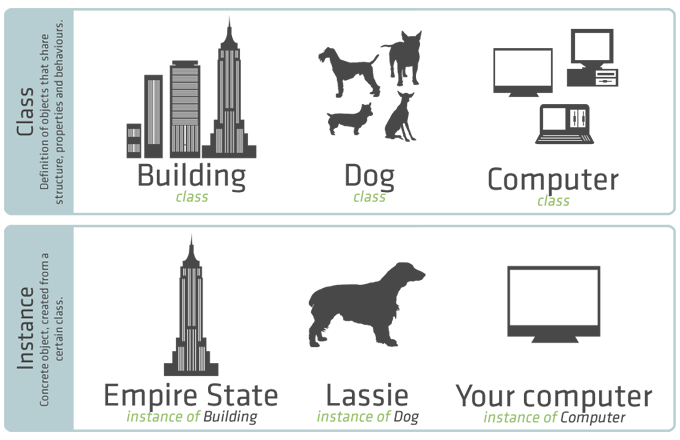
\includegraphics[width=0.8\linewidth]{figures/classes_instances.png}
  \caption{Graphical representation of a class instance.}
  \label{fig:classes}
\end{figure}

To see how classes can be defined let's try to code one representing a person:
\begin{ipython}
from datetime import date        

class Person:
\end{ipython}

First of all, if needed, we have to import the necessary modules, in this case the 
\texttt{datetime} module is used to managed the person age.
Then the \texttt{class} keyword followed by the class name is used to start the actual definition.

\subsubsection{The Constructor Method}\label{the-constructor-method}

After declaring the class name, the constructor method must be defined. In \texttt{python}, this is denoted by \texttt{\_\_init\_\_()} regardless the class name. The \texttt{\_\_init\_\_} method, as every other method in a class, takes \texttt{self} as the first argument, and then any number of parameters as desired by the programmer. The \emph{constructor} allows to specify the initial state of a class by setting its attribute values. For this example that describes a person, the programmer wants to know its name, the birthday and a job (this last one won't be initialize by the constructor though).

The \texttt{self} parameter is used to create class attributes. Variables
whose name starts with \texttt{self.} have \emph{class scope}, which means are
available within each class method. To use the parameters and
associate them with a particular instance of the class, within the
\texttt{\_\_init\_\_} method, create variables for each argument like
this: \texttt{self.variableName\ =\ param}.

\begin{ipython}
from datetime import date

# this is the class definition
# usually classes use camel naming convention
class Person:
    # the special method __init__ allows to instantiate a class
    # with an initial dataset
    def __init__(self, name, birthday):
        self.name = name
        self.birthday = birthday
        self.occupation = None # this attribute not set at instantiation
\end{ipython}

Now that we have a class definition that represents a generic person we can specialized it to some real person.

\begin{ipython}
me = Person("Matteo", date(1974, 10, 20))
print (type(me))
\end{ipython}
\begin{ioutput}
<class '\_\_main\_\_.Person'>
\end{ioutput}

When we instantiate a class, \texttt{python} first calls the \texttt{\_\_init\_\_} method and initializes the attributes with the parameter we are passing.

\subsubsection{Class Methods}

We haven't yet defined any "person behaviour", so let's add a couple of methods to our class: one computing the person's age and the other setting its primary occupation.

\begin{ipython}
class Person:
    def __init__(self, name, birthday):
        self.name = name
        self.birthday = birthday
        self.employment = None

    # this is a normal method and will work on some class attribute
    def age(self, d=date.today()):
        age = (d - self.birthday).days/365
        print ("{} is {:.0f} years old".format(self.name, age))

    def mainOccupation(self, occupation):
        self.employment = occupation
        print ("{}'s main occupation is: {}".format(self.name, self.employment))
\end{ipython}

To access class attributes and methods the dot (\texttt{.}) operator has to be used. 

\begin{ipython}
print (me.name)
\end{ipython}
\begin{ioutput}
'Matteo'
\end{ioutput}
        
\begin{ipython}
me.age(date.today())
\end{ipython}
\begin{ioutput}
Matteo is 46 years old
\end{ioutput}

\subsection{Inheritance and Overriding Methods}
\label{inheritance-and-overriding-methods}

Inheritance is basically the idea that different classes can have similar components, and in order to avoid repeating code, it is used to link parent to descendant classes. Inheritance allows the classes to share information relevant to multiple parts of the code.

For example, in a fantasy story, there are heroes and monsters but both of them are characters. Similarly dragons and orcs are monsters. Though dragons and orcs are different kind of monsters, they share some qualities: they both have a color, a size and enemies. Orcs might have characteristics that dragons do not; for example, what kind of weapon does the orc carry? (Fig.~\ref{fig:inheritance}). 

\begin{figure}[h]
  \centering
  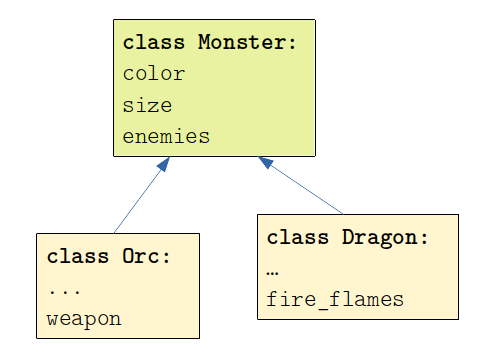
\includegraphics[width=0.5\textwidth]{figures/inheritance.png}
  \caption{Example of inheritance: both \texttt{Dragon} and \texttt{Orc} inherits from \texttt{Monster}, but both add additional attributes that qualify better each "monster features".}
  \label{fig:inheritance}
\end{figure}

Inheritance allows code to be reused and reduces the complexity of a program. The derived classes (descendants) override or extend the functionalities of the base classes (ancestors). To see how it works in more detail two derived class will be implemented from \texttt{Person}: \texttt{Adult} and \texttt{Child}.

\begin{ipython}
class Adult(Person):
    def __init__(self, name, birthday, drv_license_id):
        Person.__init__(self, name, birthday) # this is a special syntax
        self.drv_license_id = drv_license_id

class Child(Person):
    def mainOccupation(self):
        self.employment = "schoolchild"
        print ("{} is a {}".format(self.name, self.employment))
\end{ipython}

Inheritance is specified in parenthesis after the class name. \texttt{Child} still inherits from \texttt{Person} and modifies it by setting the only occupation allowed for a child, overriding the \texttt{mainOccupation} method. \texttt{Adult} class inherits from \texttt{Person} too but extends it adding a new attribute as the driving license id. 

\begin{ipython}
pippo = Adult("Goofy", date(1936, 1, 1), "A1234")
qui = Child("Huey", date(2014, 10, 9))
\end{ipython}

Behind the scenes, when instantiating a \texttt{Child} class, the constructor of \texttt{Person} is called and the attributes, \texttt{name} and \texttt{birthday} are still initialised.  

For the \texttt{Adult} class things are a little bit different because a new attribute has been added, so we need to code its own constructor where we first call explicitly the \texttt{Person}'s constructor (\texttt{Person.\_\_init\_\_(self, \ldots)} and then we initialise the new attribute.

\begin{ipython}
pippo.age()
pippo.mainOccupation("Comic's character")
\end{ipython}
\begin{ioutput}
Goofy is 85 years old
Goofy's main occupation is: Comic's character
\end{ioutput}

\begin{ipython}
qui.age()
qui.mainOccupation()
\end{ipython}
\begin{ioutput}
Huey is 6 years old
Huey is a schoolchild
\end{ioutput}

\section*{Exercises}
\cprotEnv\begin{question}
Take the code for the Black-Scholes formula from exercise~\ref{ex:BS1} and wrap it in a function. Then, use this function to calculate the prices of calls with various strikes, using the following input data.

\begin{ipython}
s = 800 
# strikes expressed as % of spot price
moneyness = [0.5, 0.75, 0.825, 1.0, 1.125, 1.25, 1.5]
vol = 0.3
ttm = 0.75
r = 0.005
\end{ipython}

The output should be a dictionary mapping strikes to call prices.
\end{question}

\cprotEnv\begin{solution}
\begin{ipython}
from math import log, exp, sqrt
from scipy.stats import norm

def d1(St, K, r, vol, ttm):
    num = log(St/K) + (r + 0.5*pow(vol, 2)) * ttm
    den = vol * sqrt(ttm)
    return num/den

def d2(St, K, r, vol, ttm):
    return d1(St, K, r, vol, ttm) - vol*sqrt(ttm)

def call(St, K, r, vol, ttm):
    return St * norm.cdf(d1(St, K, r, vol, ttm)) - K * exp(-r*ttm)*norm.cdf(d2(St, K, r, vol, ttm))

s = 800
# strikes expressed as % of spot price
moneyness = [0.5, 0.75, 0.825, 1.0, 1.125, 1.25, 1.5]
vol = 0.3
ttm = 0.75
r = 0.005

result = {}
for m in moneyness:
    result[s*m] = call(s, m*s, r, vol, ttm)
print(result)

{400.0: 401.66074527896365,
  600.0: 213.9883852521275,
  660.0: 166.85957363897393,
  800.0: 84.03697017660357,
  900.0: 47.61880394696229,
  1000.0: 25.632722952585738,
  1200.0: 6.655275227771156}
\end{ipython}
\end{solution}

\cprotEnv\begin{question}
Write two classes, \texttt{Circle} and \texttt{Rectangle} that given the radius and height, width respectively allow to compute area and perimeter of the two shapes. Test them with the following:

\begin{ipython}
a_circle = Circle(5)
print("My circle has an area of {} m2".format(a_circle.area()))

a_rectangle = Rectangle(3, 6)
print ("My rectangle has a perimeter of {} m and an area of {} m2".format(a_rectangle.perimeter(), a_rectangle.area())}
\end{ipython}
\end{question}

\cprotEnv\begin{solution}
\begin{ipython}
from math import pi

class Circle:
    def __init__(self, radius):
        self.radius = radius

    def area(self):
        return pi*self.radius**2

class Rectangle:
    def __init__(self, width, height):
        self.height = height
        self.width = width

    def area(self):
        return self.width*self.height

    def perimeter(self):
        return self.width*2 + self.height*2

circle = Circle(5)
print ("My circle area is {:.1f} m**2".format(circle.area()))

rect = Rectangle(3, 6)
print ("My rect area is {:.1f} m**2 and the perimeter is {} m".format(rect.area(), rect.perimeter()))

My circle area is 78.5 m**2
My rect area is 18.0 m**2 and the perimeter is 18 m
\end{ipython}
\end{solution}

\cprotEnv\begin{question}
Define a class \texttt{Songs}, its \texttt{\_\_init\_\_} should take as input a dictionary (\texttt{lyrics} that contains lyrics line by line). Define a method, \texttt{sing\_me\_a\_song} that prints each element of the lyrics in his own line. Also test it with the following input.

\begin{ipython}
lyrics = {"Wonderwall":["Today is gonna be the day",
	                    "That they're gonna throw it back to you",
	                    "By now you should've somehow", "..."],
	      "Wish you were here": ["So, so you think you can tell",
                                 "Heaven from hell",
	                             "Blue skies from pain", "..."]}
\end{ipython}
\end{question}

\cprotEnv\begin{solution}
\begin{ipython}
class Songs:
    def __init__(self, lyrics):
        self.lyrics = lyrics

    def sing_me_a_song(self, title):
        song = self.lyrics[title]
        print ("Title: {}".format(title))
        print ("********************")
        for line in song:
            print (line)

lyrics = {"Wonderwall":["Today is gonna be the day",	
	                    "That they're gonna throw it back to you",
	                    "By now you should've somehow", "..."],
	      "Wish you were here": ["So, so you think you can tell",
                        "Heaven from hell",
                        "Blue skies from pain", "..."]}

songs = Songs(lyrics)
songs.sing_me_a_song("Wonderwall")

Title: Wonderwall
********************
Today is gonna be the day
That they're gonna throw it back to you
By now you should've somehow
...
\end{ipython}
\end{solution}

\begin{question}
Define a Point2D class that represent a point in a plane. Its \texttt{\_\_init\_\_} method should accept the point coordinates \texttt{x} and \texttt{y}. Write a method \texttt{distanceTo} that compute the distance of the point to another passed as input. Test the class by printing the distance of the point \(P=(4, 5)\) to the origin \(P=(0,0)\) and to \(P=(3,4)\).

\noindent\textbf{Hint:} in the Cartesian plane the distance between two points is: $\sqrt{(x_1 - x_2)^2 + (y_1 - y_2)^2}$.
\end{question}

\cprotEnv\begin{solution}
\begin{ipython}
from math import sqrt

class Point2D:
    def __init__(self, x, y):
        self.x = x
        self.y = y

    def distanceTo(self, x, y):
        dist = sqrt((self.x-x)**2 + (self.y - y)**2)
        return dist

    def distanceTo_v2(self, p):
        dist = sqrt((self.x-p[0])**2 + (self.y - p[1])**2)
        return dist

    def distanceTo_v3(self, p):
        dist = sqrt((self.x-p.x)**2 + (self.y - p.y)**2)
        return dist

point = Point2D(4, 5)
p0 = (0, 0)
point0 = Point2D(0, 0)
print ("distance to p0: {:.2f}".format(point.distanceTo(p0[0], p0[1])))
print ("distance_v2 to p0: {:.2f}".format(point.distanceTo_v2(p0)))
print ("distance_v3 to p0: {:.2f}".format(point.distanceTo_v3(point0)))
p1 = (3, 4)
point1 = Point2D(3, 4)
print ("distance to p1: {:.2f}".format(point.distanceTo(p1[0], p1[1])))
print ("distance_v2 to p1: {:.2f}".format(point.distanceTo_v2(p1)))
print ("distance_v3 to p1: {:.2f}".format(point.distanceTo_v3(point1)))

distance to p0: 6.40
distance\_v2 to p0: 6.40
distance\_v3 to p0: 6.40
distance to p1: 1.41
distance\_v2 to p1: 1.41
distance\_v3 to p1: 1.41
\end{ipython}
\end{solution}

\cprotEnv\begin{question}
Write a class \texttt{Student} which inherits from the class \texttt{Person} defined in Chapter Object Oriented Programming in Python. This new class should have two new attributes: \texttt{grade} which keeps the type of school and \texttt{votes} a dictionary which will record the student's votes and the corresponding course. Then add two methods, one to add votes and another to compute the average vote.Instantiate a "student" add some votes and show how good it has been.

\noindent\textbf{Hint:} this is the \texttt{Person} class already developed.

\begin{ipython}
class Person:
    def __init__(self, name, birthday):
        self.name = name
        self.birthday = birthday
        self.employment = None

    def age(self, d=date.today()):
        age = (d - self.birthday).days/365
        print ("{} is {:.0f} years old".format(self.name, age))

    def mainOccupation(self, occupation):
        self.employment = occupation
        print ("{}'s main occupation is: {}".format(self.name, self.employment))
\end{ipython}
\end{question}

\cprotEnv\begin{solution}
\begin{ipython}
class Student(Person):
    def __init__(self, name, birthday, school):
        Person.__init__(self, name, birthday)
        self.grade = school
        self.votes = {}

    def addVote(self, subject, vote):
        self.votes[subject] = vote

    def average(self):
        print ("List of votes")
        print ("-------------")
        for k, v in self.votes.items():
            print ("{}: {}".format(k, v))
        avg = sum(self.votes.values())/len(self.votes)
        print ("-------------")
        print ("Avg: {:.1f}".format(avg))

student = Student("Mario", date(1980, 5, 6), "Liceo Scientifico G. Galilei")
student.addVote("Calculus", 8)
student.addVote("Literature", 5.5)
student.addVote("Latin", 6.5)
student.average()

List of votes
-------------
Calculus: 8
Literature: 5.5
Latin: 6.5
-------------
Avg: 6.7
\end{ipython}
\end{solution}


\begin{thebibliography}{9}
\bibitem{OOP} \href{https://realpython.com/python3-object-oriented-programming/}{\emph{Tutorial on Object Oriented Programming}}, Real Python [Online]
\end{thebibliography}
